
\documentclass{article}
\usepackage{graphicx} % Required for inserting images
\usepackage{fancyhdr} % Required for header and footer configuration
\usepackage[a4paper, margin=2.5cm, left=1.5cm, right=1.5cm, bottom=4cm]{geometry} % Required for setting page margins
\usepackage[T1]{fontenc}
\usepackage[default,oldstyle,scale=1]{opensans} % Utilizzo del font Open Sans
\usepackage{lipsum}
\usepackage{makeidx}
\usepackage{booktabs}
\usepackage{tabularray}
\usepackage[colorlinks=true, linkcolor=black, urlcolor=blue, citecolor=blue]{hyperref}
\usepackage{tabularx}
\usepackage{makecell}
\usepackage{enumitem} % Pacchetto per la personalizzazione degli elenchi
\usepackage{booktabs}
\usepackage{subcaption}
\usepackage{pgfplots}
\usepgfplotslibrary{dateplot} % Per gestire gli assi con date

% Configure header and footer for the first page
\fancypagestyle{firstpage}{
    \fancyhf{} % Clear header and footer
    \renewcommand{\headrulewidth}{0pt} % Remove header rule line
    \lhead{} % Header on the left
    \chead{} % Header in the center
    \rhead{} % Header on the right
    \lfoot{} % Footer on the left
    \cfoot{\vspace{5pt}\\\hrulefill\\\vspace{10pt}\textbf{BeeLive}\\Gruppo 21} % Footer in the center
    \rfoot{\vspace{32.5pt}\\\thepage} % Footer on the right
}

% Configure header and footer for non-plain pages (second page onwards)
\fancypagestyle{nonplain}{
    \fancyhf{} % Clear header and footer
    \lhead{} % Header on the left
    \chead{} % Header in the center
    \rhead{
\includegraphics[width=2cm]{Images/BeeLive-Logo.png}\\\vspace{2pt}} % Header on the right
    \lfoot{} % Footer on the left
    \cfoot{\vspace{5pt}\\\hrulefill\\\vspace{10pt}\textbf{BeeLive}\\Gruppo 21} % Footer in the center
    \rfoot{\vspace{32.5pt}\\\thepage} % Footer on the right
}

% Adjust vertical space between header and text                                    
\setlength{\headsep}{65pt} 
% Adjust vertical space between text and footer
\setlength{\footskip}{0pt} 

\title{
\includegraphics[width=0.75\textwidth]{Images/BeeLive-Logo.png}\\\vspace{100pt}
\LARGE{\textbf{BeeLive\\Deliverable 4}}}
\author{Gruppo 21:\\
Cipriani Pietro, 226959\\
Orlando Dennis, 227688\\
Ziviani Elia, 228172}
\date{22 Aprile 2024}

\makeindex % Indica che vogliamo creare un indice

\begin{document}

\maketitle
\thispagestyle{firstpage} % Apply firstpage style to the first page
\clearpage

\pagestyle{nonplain} % Apply non-plain style to subsequent pages

\renewcommand{\contentsname}{Indice}
\tableofcontents

\clearpage

\section{Revisione}
...

\section{Introduzione}

\subsection{Componenti del gruppo}
\begin{itemize}
    \item Cipriani Pietro, matricola 226959, \lbrack\href{https://github.com/pietrocipriani}{github profile}\rbrack
    \item Orlando Dennis, matricola 227688, \lbrack\href{https://github.com/dennisorlando}{github profile}\rbrack
    \item Ziviani Elia, matricola 228172, \lbrack\href{https://github.com/ELI20ZIVI}{github profile}\rbrack
\end{itemize}

\subsection{Scopo del progetto}

Lo scopo del progetto 'BeeLive' è quello di risolvere il problema riguardante la difficoltà nel reperire informazioni riguardanti gli eventi che influenzano la viabilità all'interno del Comune di Trento. Prevediamo un sistema informativo, dedicato agli utenti cittadini, che mostri visualmente le variazioni della viabilità in città, informando gli stessi di eventuali modifiche che potrebbero colpirli direttamente.

\subsection{Link utili}
Il primo link fornito è quello della repository github. La repository è stata creata appena il corso è cominciato, infatti inizialmente è risultata utile al fine di scrivere in modo collaborativo i primi deliverable.\\
E' stato deciso di integrare in questa repository anche le fasi di sprint in quanto come team riteniamo utile la possibilità di accedere alla documentazione redatta nei primi due deliverable.\\
La repository è accessibile al seguente link: \href{https://github.com/ELI20ZIVI/BeeLive/}{Repository GitHub}\\ \\
Il secondo link fornito è quello di Apiary. Apiary è uno strumento che permette di creare e documentare in modo molto accurato e approfontido le API utilizzate nel progetto.\\
Il link di Apiary è il seguente: \href{https://beelive.docs.apiary.io/#}{Link Apiary}\\ \\
Per eseguire un deploy del progetto sarà necessario installare i due applicativi (Mobile e Desktop). Il link per scaricarli e testarli è \href{github-release-page}.\\
Gli account da utilizzare per il login sono i seguenti:
\begin{itemize}
    \item Utente Autorizzato: Username: \textit{user1}, Password: \textit{password1}
    \item Utente Amministratore: Username: \textit{user2}, Password: \textit{password2}
    \item L'utente comune non necessita di credenziali di accesso
\end{itemize}

\clearpage

\section{Sezione generale}

\subsection{Strategia di Branching}
Anche per questo secondo sprint è stata evitata la strategia di branching "Master only", infatti come descritto nel documento "Deliverable 3", per noi la creazione e l'utilizzo di un unico branch principale \textit{main} avrebbe causato problemi di collaborazione e conflitti nel momento in cui tutti i componenti lavoravano conteporaneamente a stesse sezioni del progetto. \\

\noindent
Abbiamo quindi deciso di mantenere la stessa metodologia di branching dello scorso sprint, ossia una \textit{Feature Branching} con però un branch \texttt{develop}, precedente al branch \texttt{main}, sul quale una volta ritenute soddisfacenti le modifiche e le feature aggiunte, queste vengono integrate.\\
Quando le features sono tutte integrate nel branch \texttt{develop}, questo viene, una volta testato sia tutto funzionante nei minimi dettagli, integrato nel branch \texttt{main} come operazione di 'release'.\\

\noindent
Tramite questo approccio puntiamo ad incrementare la collaborazione tra i membri del team, ridurre i conflitti e le inconsistenze nel codice, facilitare la gestione delle diverse attività in corso e mantenere inoltre una mappatura di tutte le diverse modifiche e progressi del progetto, mantenendo ben strutturata la storia del codice.\\

Segue una lista dei branch utilizzati per lo sviluppo del progetto; da notare che molte di queste branches sono state eliminate una volta integrate in \texttt{develop}, per cui su github potrebbero non apparire.

\subsubsection{\texttt{main}}

Il branch principale del progetto, in cui vengono integrate tutte le funzionalità completate e testate.\\
Tutte le funzionalità all'interno di questo branch sono considerate terminate e funzionanti, pronte per essere rilasciate.

\subsubsection{\texttt{develop}}

Il branch di sviluppo del progetto, in cui vengono integrate tutte le funzionalità completate e testate.\\
Non e' pensato propriamente come il branch in cui vengono rilasciate le funzionalita' ma piuttosto come un branch di supporto per il branch principale, infatti in questo branch vengono prima caricate le funzionalita' dagli altri branch specifici e successivamente testate.\\
Una volta che sono considerate funzionanti sono quindi integrate nel branch principale.

\subsubsection{\texttt{preview}}

Branch dedicato alla preview dell'interfaccia grafica dei due applicativi.\\
E' stato utilizzato al momento della prima presentazione del progetto per mostrare il lavoro svolto ai committenti e per ricevere feedback su eventuali modifiche da apportare.\\
Integra dei mockup delle varie interfacce, desktop e mobile, che andranno sviluppate.\\
Parte della preview è stata poi utilizzata in \texttt{da\_frontend} come punto di partenza per l'interfaccia,

\subsubsection{\texttt{deliverable}}

Branch dedicato alla stesura dei vari documenti di deliverable.\\
Creato per mantenere separata la stesura della documentazione dal codice sorgente e per rispettare la metodologia di branching.

\subsubsection{\texttt{refactoring}}

Questo branch nasce per la necessità di effettuare un refactoring del codice. Prima di eseguire il merge in \texttt{main} spesso risulta necessario effettuare delle modifiche al codice per renderlo più leggibile, mantenibile e performante.\\
Avendo un ambiente separato si annulla la possibilità di introdurre errori nel codice principale.

\subsubsection{\texttt{deployment}}

Branch dedicato alla preparazione del deploy del progetto.\\
Vengono preparate tutte le componenti alla fase di deploy, come la creazione dei file di configurazione, la preparazione dei file per il deploy e la creazione di script per automatizzare il deploy.

\subsubsection{\texttt{management-server}}

Branch dedicato allo sviluppo del server di gestione, il server utilizzato dall'applicativo desktop (Quindi dagli utenti autorizzati) per eseguire tutte le operazioni di gestione degli eventi.

\subsubsection{\texttt{public\_server}}

Similmente al branch precedente, questo branch è dedicato allo sviluppo del server pubblico, il server utilizzato dall'applicativo mobile (Quindi dagli utenti comuni) per la visualizzazione degli eventi e le varie impostazioni dell'applicativo.

\subsubsection{\texttt{da\_frontend}}

Branch dedicato allo sviluppo dell'interfaccia grafica dell'applicativo desktop.\\
In questo branch vengono sviluppate tutte le componenti che caratterizzano l'interfaccia grafica dell'applicativo desktop.

\subsubsection{\texttt{da\_authn}}

...

\subsubsection{\texttt{da\_event\_list}}

Branch di sviluppo della funzionalità di visualizzazione a lista degli eventi a disposizione dell'utente in questione sull'applicativo desktop.\\
E' integrata tutta la logica di richiesta delle informazioni al server e di visualizzazione delle stesse in modo chiaro e ordinato.

\subsubsection{\texttt{ma\_client}}

Branch dedicato allo sviluppo del client mobile, i.e. l'applicazione mobile utilizzata dagli utenti comuni (autenticati e non) che intendono visualizzazione le criticita' presenti in citta'.\\
Il branch, una volta concluso lo sviluppo dell'applicativo, e' stato integrato nel branch \texttt{develop} per i test in associata con tutti gli altri moduli.


\subsubsection{\texttt{ma\_screen}}

Branch dedicato alla creazione delle schermate dell'applicativo mobile, i.e. tutte le schermate che l'utente visualizzera' durante l'utilizzo dell'applicativo.\\
Questo branch è stato integrato in \texttt{ma\_client} in quanto sua dipendenza.

\subsubsection{\texttt{ma\_details}}

Branch dedicato allo sviluppo dell'interfaccia di visualizzazione degli eventi e dei rispettivi sottoeventi sull'applicativo mobile.

\subsubsection{\texttt{ma\_map}}

Branch utilizzato per sviluppare la libreria che permette di integrare la mappa all'interno dell'applicativo mobile.\\
Questa libreria permette di visualizzare in modo chiaro e intuitivo le criticita' presenti in citta' e di visualizzare la posizione degli eventi.

\subsubsection{\texttt{ws-fetch-event}}

Branch dedicato allo sviluppo del webserver pubblico, i.e. il webserver in cui sono stati implementati gli endpoint API dedicati al fetching di eventi ad opera dell'applicativo mobile.\\
Una volta che il modulo e' stato completato, e' stato integrato nel branch \texttt{develop} per i test con tutti gli altri moduli.

\subsubsection{\texttt{ws-insert-event}}

Branch dedicato allo sviluppo del webserver gestionale, i.e. il webserver in cui sono stati implementati gli endpoint API dedicati all'inserimento degli eventi all'interno del sistema ad opera dell'applicativo desktop. \\
Utile allo sviluppo del modulo utilizzato dall'applicativo desktop per l'inserimento delle criticita' in citta'.
Una volta che il modulo e' stato completato, e' stato integrato nel branch \texttt{develop} per i test con tutti gli altri moduli.\\
Delle versioni intermedie di questa branch sono state usate da altre branches, in particolare da \texttt{da\_desktop}, in quanto necessaria per effettuare il testing di quest'ultima.

\clearpage

\subsection{Product Backlog}
Nella pagina seguente vi è riportato il product backlog che abbiamo sviluppato per questo progetto. E' possibile notare una linea di demarcazione che limita inferiormente le entries selezionate per il primo sprint.

\begin{table}[!ht]
    \centering
    \renewcommand{\arraystretch}{1.3} % Imposta lo spazio verticale delle righe
    \begin{tabularx}{\textwidth}{| r | X | r | r |}
        \Xhline{2pt}
        \makecell{\textbf{Nome}} & \makecell{\textbf{User story}} & \makecell{\textbf{Priorità}} & \makecell{\textbf{Stima}} \\
        \Xhline{2pt}
        \makecell{Visualizzazione\\eventi in città} & \makecell{Da utente, voglio visualizzare la lista degli eventi in città} & \makecell{200} & \makecell{8}\\
        \hline
        \makecell{Aggiunta eventi\\da utente\\autorizzato} & \makecell{Da utente autorizzato, devo essere in grado di aggiungere degli eventi\\in modo da comunicare la loro presenza agli utenti} & \makecell{190} & \makecell{8}\\
        \hline
        \makecell{Registrazione e\\accesso all'\\app mobile} & \makecell{Da utente, voglio avere la possibilità di accedere ad una\\visualizzazione e descrizione più dettagliata di un evento in modo da\\conoscere meglio le specifiche di tale evento} & \makecell{180} & \makecell{8}\\
        \hline
        \makecell{Visualizzazione\\criticità\\su mappa} & \makecell{Da utente, voglio visualizzare su una cartina le zone colpite dai diversi\\eventi, in modo da capire visivamente se in una zona che mi\\interessa vi è un evento attivo} & \makecell{170} & \makecell{6}\\
        \hline
        \makecell{Accesso alle\\criticità e ai\\loro dettagli} & \makecell{Da utente, voglio essere in grado di visualizzare la lista\\delle criticità presenti in città} & \makecell{160} & \makecell{8}\\
        \Xhline{2pt}
        \makecell{Impostazione\\categorie\\d'interesse\\per gli eventi} & \makecell{Da utente, voglio essere in grado di impostare le categorie di eventi\\alle quali io sono interessato, in modo che la lista di eventi visibile\\dall'applicazione contenga solamente gli eventi che mi interessano,\\e in modo che io non venga notificato di alcun evento\\che io non ritenga appartenere ad una categoria interessante} & \makecell{100} & \makecell{5}\\
        \hline
        \makecell{Impostazione\\zone\\d'interesse} & \makecell{Da utente, voglio essere in grado di impostare delle zone di interesse,\\in modo che io venga notificato di qualsiasi evento che insorga\\in una di queste zone} & \makecell{90} & \makecell{7}\\
        \hline
        \makecell{Visualizzazione\\eventi\\di competenza} & \makecell{Da utente autorizzato, devo essere in grado di visualizzare gli eventi\\di mia competenza, in modo da sapere quali eventi sono stati creati e\\monitorare il loro stato} & \makecell{80} & \makecell{5}\\
        \hline
        \makecell{Modifica\\eventi} & \makecell{Da utente autorizzato, devo essere in grado di modificare degli eventi\\in modo da evitare errori comunicativi} & \makecell{75} & \makecell{2}\\
        \hline
        \makecell{Accesso\\account\\utente} & \makecell{Da utente registrato, voglio essere in grado di poter accedere al\\mio account in modo da poter riottenere le aree di interesse e\\le impostazioni che ho precedentemente salvato} & \makecell{70} & \makecell{3}\\
        \hline
        \makecell{Visualizzazione\\eventi\\di categorie\\di interesse} & \makecell{Da utente, voglio essere in grado di visualizzare solo\\eventi di categorie di interesse} & \makecell{60} & \makecell{3}\\
        \hline
        \makecell{Selezione\\percorso} & \makecell{Da utente, voglio essere in grado di selezionare un percorso a partire\\da dei waypoint, per impostare dei percorsi di interesse} & \makecell{40} & \makecell{2}\\
        \hline
        \makecell{Eliminazione\\eventi} & \makecell{Da utente autorizzato, devo essere in grado di eliminare degli eventi} & \makecell{40} & \makecell{2}\\
        \hline
    \end{tabularx}
    \caption{Product backlog}
\end{table}

\clearpage

\subsection{Definition of "Done"}
La seguente 'Definition of Done' è basata su una valutazione collettiva che ha preso in considerazione  diversi fattori riguardanti la qualità del lavoro, non ignorando però la fattibilità e la realizzabilità di questi.\\
I criteri inclusi nella nostra 'Definition of Done' definita per il progetto sono i seguenti:
\begin{itemize}
	\item \textbf{Funzionalità}: le funzionalità che il codice implementa devono soddisfare appieno l'usecase / gli usecase associati al codice.
    \item \textbf{Codice}: Il codice deve essere revisionato e la sua correttezza / adeguatezza approvata da almeno un altro membro del team.
    \item \textbf{Test}: Il codice deve essere adeguatamente coperto da test unitari, di integrazione e funzionali, che devono essere scritti e superati con successo. Un adeguato numero di questi test deve essere scritto da membri diversi.
    \item \textbf{Documentazione}: Il codice e le funzionalità implementate devono essere adeguatamente documentati. Questo giudizio di adeguatezza deve essere dato da almeno un altro membro del team.
    \item \textbf{Build e Deployment}: Il codice deve integrarsi con successo nella build principale e la sua inclusione nella build principale non deve assolutamente far fallire dei test, nel caso in cui quest'ultimi venivano correttamente superati priva dell'inclusione.
    \item \textbf{Performance}: le funzionalità e il codice introdotti non devono causare visibili degradi alle performance di nessun elemento del progetto.
    \item \textbf{Conformità}: Il prodotto deve essere conforme alle normative legali e agli standard di sicurezza e qualità specifici del settore.
\end{itemize}

\clearpage

\section{Sezione Sprint \#2}

\subsection{Goal dello sprint}


\subsection{Sprint Planning}
\textbf{User story}: 

\textbf{Product backlog}
\begin{table}[htbp]
    \centering
    \renewcommand{\arraystretch}{1.3} % Imposta lo spazio verticale delle righe
    \begin{tabularx}{\textwidth}{| X | r | r | r | r |}
        \Xhline{2pt}
        \makecell{\textbf{Nome}} & \makecell{\textbf{User story}} & \makecell{\textbf{Cosa fare}} & \makecell{\textbf{Assegnazione}} & \makecell{\textbf{Stima}} \\
        \Xhline{2pt}
        \makecell{} & \makecell{} & \makecell{} & \makecell{} & \makecell{} \\
        \hline
    \end{tabularx}
    \caption{Product backlog user story 1}
\end{table}

\subsection{Burndown chart}
Il burndown chart è uno strumento utilizzato per monitorare il progresso di un progetto.\\
Giorno per giorno si può visualizzare l'andamento dei lavori e capire se si sta procedendo secondo i piani o se ci sono ritardi.\\

\begin{figure}[htbp]
    \centering
    \begin{tikzpicture}
        \begin{axis}[
            width=12cm, height=8cm, % Dimensioni del grafico
            date coordinates in=x,
            xlabel={Date},
            ylabel={Tasks Remaining},
            xticklabel={\day-\month},
            grid=major,
            legend pos=north east,
        ]
        \addplot[
            color=blue,
            mark=square*,
            thick
        ] table [col sep=comma, x=date, y=planned] {
            date, planned
            2024-05-01, 122
            2024-05-16, 0
        };
        \addlegendentry{Planned}

        \addplot[
            color=red,
            mark=triangle*,
            thick
        ] table [col sep=comma, x=date, y=actual] {
            date, actual
            2024-05-01, 122
            2024-05-02, 117
            2024-05-03, 115
            2024-05-04, 113
            2024-05-05, 109
            2024-05-06, 96
            2024-05-07, 83
            2024-05-08, 79
            2024-05-09, 76
            2024-05-10, 74
            2024-05-11, 65
            2024-05-12, 60
            2024-05-13, 48
            2024-05-14, 42
            2024-05-15, 42
            2024-05-16, 42
        };
        \addlegendentry{Actual}
        \end{axis}
    \end{tikzpicture}
    \caption{Burndown Chart}
    \label{fig:burndown}
\end{figure}

\clearpage

\subsection{Test cases}
\subsubsection{Test cases per il modulo \texttt{public\_server}}
Il modulo \texttt{public\_server} è il modulo che si occupa di gestire le richieste provenienti dall'applicativo mobile.\\
Infatti ha il compito di gestire tutte le richieste provenienti dagli applicativi mobile installati sui dispositivi, andando quindi a reperire dal database tutti gli eventi che sono richiesti nella richiesta stessa.\\

\begin{itemize}
    \item Test case :
\end{itemize}

\begin{table}[htbp]
    \centering
    \renewcommand{\arraystretch}{1.3} % Imposta lo spazio verticale delle righe
    \begin{tabularx}{\textwidth}{| r | X | X | X | X | X | X |}
        \Xhline{2pt}
        \makecell{\textbf{No.}} & \makecell{\textbf{Descrizione}} & \makecell{\textbf{Dati}} & \makecell{\textbf{Precondizioni}} & \makecell{\textbf{Risultati attesi}} & \makecell{\textbf{Note}} \\
        \Xhline{2pt}
         &  &  &  &  &  \\
        \hline
    \end{tabularx}
\end{table}

\subsubsection{Test cases per il modulo \texttt{management\_server}}
Il modulo \texttt{management\_server} è il modulo che si occupa di gestire le richieste provenienti dall'applicativo desktop.\\
Infatti ha il compito di gestire tutte le richieste provenienti dagli applicativi desktop installati sui dispositivi degli utenti autorizzati, per permettere di poter eseguire tutte le operazioni sugli eventi disponibili.

\begin{itemize}
    \item Test case :
\end{itemize}

\begin{table}[htbp]
    \centering
    \renewcommand{\arraystretch}{1.3} % Imposta lo spazio verticale delle righe
    \begin{tabularx}{\textwidth}{| r | X | X | X | X | X | X |}
        \Xhline{2pt}
        \makecell{\textbf{No.}} & \makecell{\textbf{Descrizione}} & \makecell{\textbf{Dati}} & \makecell{\textbf{Precondizioni}} & \makecell{\textbf{Risultati attesi}} & \makecell{\textbf{Note}} \\
        \Xhline{2pt}
         &  &  &  &  &  \\
        \hline
    \end{tabularx}
\end{table}

\subsection{Sprint review}

\subsection{Product backlog refinement}

\subsection{Sprint retrospective}

\subsection{Deploy}

\section{Sezione finale}
\subsection{Diagramma del deploy finale}

\subsection{Stack tecnologico usato}

\subsection{Conclusioni}

\end{document}
